\documentclass[
reprint,amsmath,amssymb,aps]{revtex4-2}

\usepackage{graphicx}
\usepackage{dcolumn}
\usepackage{bm}
\usepackage{float}
\usepackage{tabularx}
\usepackage{multirow}
\usepackage{braket}
\usepackage{amsmath}


\begin{document}

\preprint{APS/123-QED}

\title{Spin dynamics and magnetic bistability in single Dy adatoms on graphene/Ir(111)
studied by SP-STM}

\author{A. Curcella}
 \email{Equally contributed to this work} 
\affiliation{Institute of Physics, Ecole Polytechnique Fédérale de Lausanne, CH-1015 Lausanne, Switzerland}

\author{D. Sblendorio}
 \email{equally contributed to this workw}
\affiliation{Institute of Physics, Ecole Polytechnique Fédérale de Lausanne, CH-1015 Lausanne, Switzerland}

\author{S. Rusponi}
\affiliation{Institute of Physics, Ecole Polytechnique Fédérale de Lausanne, CH-1015 Lausanne, Switzerland}

\author{M. Pivetta}
\affiliation{Institute of Physics, Ecole Polytechnique Fédérale de Lausanne, CH-1015 Lausanne, Switzerland}

\author{F. Patthey}
\affiliation{Institute of Physics, Ecole Polytechnique Fédérale de Lausanne, CH-1015 Lausanne, Switzerland}

\author{H. Brune}
\affiliation{Institute of Physics, Ecole Polytechnique Fédérale de Lausanne, CH-1015 Lausanne, Switzerland}
 

\begin{abstract}
ABSTRACT
% The magnetic stability in single Dy adatoms on graphene/Ir(111) is investigated by means of spin-polarized scanning tunneling microscopy at liquid He temperature. Telegraph-noise traces demonstrate the bistability of the Dy magnetization, and exhibit long relaxation times of several minutes, consistent with previous XMCD measurements \citep{baltic2016}.
% The asymmetric occupancy of the magnetic states as a function of tunnel voltage is evidence for a spin-torque exerted by tunneling electrons on the single-atom magnet \citep{Khajetoorians2013,delgado2010}.
% Based on existing theoretical works, we implement a model that quantitatively reproduces the asymmetry in the occupancy of the magnetic states and their average lifetimes, the temperature dependence of the magnetization reversal, and the value of the magnetoresistive contribution in the STM current. 
\end{abstract}

\maketitle

\section{Introduction}
% Manipulation of the magnetic states of nano-objects and in surface adsorbed single adatoms offer novel avenues for exploring the fundamental physics that determine their behavior. Understanding this behavior is essential for the development of future spintronic devices and the realization of ultra-high-density magnetic memory [citations...]. The injection of a spin-polarized current can efficiently reorient the magnetization of a nanomagnet \citep{Khajetoorians2013,krause_joule_2011,loth2010}, enabling the possibility of reading and writing of the magnetic states.
% Dysprosium atoms adsorbed on a single graphene layer grown on Ir(111) were identified as stable single-atom magnets \citep{baltic2016}. Previous scanning tunneling microscopy (STM) studies revealed these atoms self assemble into a highly-ordered superlattice after annealing at 40~K \citep{baltic2016,pivetta2018}. Obtaining uniformly dispersed bistable magnetic nanostructures on a decoupling atomic layer is a paramount achievement for the development of ultra-high magnetic memory densities [citations]. Previous x-ray magnetic circular dichroism (XMCD) measurements revealed that Dy adatoms on graphene/Ir(111) possess a \textit{4f$^{\:10}$} occupation, a \textit{J} = 8 total angular momentum identical to Dy in the gas phase, and a \textit{J$_z$} = $\pm$7 out-of-plane magnetic ground state \citep{baltic2016,baltic2018}.
% The measured spin lifetimes are of the order of 1000~s at 2.5~K.
% However, the lifetimes obtained by XMCD are limited by the interaction of the adatoms with photon-induced secondary electrons. The extrapolation of the intrinsic magnetization lifetime at zero photon flux represents a lower bound estimate.
\section{Results}
Here we present the results of SP-STM conducted on well-isolated Dy adatoms adsorbed on Gr/Ir(111). To interpret the experimental results, we implement a model which accounts for the recently observed intra-atomic interaction between internal \textit{4f} and external \textit{6s-5d} polarized shells \cite{pivetta2020}; offering an original revision of the description of the spin dynamics in rare-earth based single-adatom magnets. The Dy adatoms adsorb onto the 6-fold symmetrical ($C_{6v}$) graphene hollow site \cite{baltic2018}. The crystal field lifts the degeneracy of the magnetic states and gives rise to a strong out-of-plane easy-axis anisotropy.
If the intra-atomic exchange is neglected (\textit{i.e.} the external shells are not polarized), the magnetic states $\ket{M}$ are defined solely by the spin of the \textit{4f} shell $\ket{M}=\ket{j_{4f}}$ (Fig.~\ref{fig:intra}a). The zero-field level scheme of Dy system, in this case, is depicted in Fig.~\ref{fig:intra}b. The term $B_6^6$ in the crystal field Hamiltonian term (see Supplemental) mixes the states with $\Delta j_{4f}=6n$, with $n\in \mathbb{Z}$. The states $\ket{j_{4f}}=\ket{\pm 6}$ are therefore mixed, with a splitting of $\omega=1.3 10^{-2}$ meV. The mixing of these states permits the only efficient channel for magnetization reversal, via quantum tunnelling of magnetization (QTM), at energies $E<20$ meV \citep{baltic2016}. The inclusion of the intra-atomic exchange term in the Hamiltonian (\textit{i.e.} the external shells are polarized), produces a modified level scheme. In addition to the spin of the \textit{4f} shell, the new basis includes the spin of the valence \textit{5d}-\textit{6s} shell $\ket{M}=\ket{m_i}=\ket{j_{4f},s_{5d},s_{6s}}$ (Fig.~\ref{fig:intra}d). The intra-atomic exchange couples the \textit{4f} and the \textit{5d}-\textit{6s} shells ferromagnetically (Fig.~\ref{fig:intra}f) \cite{pivetta2020}. 
In this new basis, the $B_6^6$ term of the crystal field mixes the states with $\Delta M_{tot}=\Delta j_{4f} + \Delta s_{5d} + \Delta s_{6s}=6n$, $n\in \mathbb{N}$. This results in the mixing and splitting of the states $\ket{M}=\ket{m_{\pm 5}}$ and $\ket{M}=\ket{m_{\pm 8}}$ (Fig.~\ref{fig:intra}e), which have $\Delta M_{tot}\sim 10+1+1 = 12$ and $\Delta M_{tot}\sim 16 +1+1=18$, respectively. With respect to the former case, two magnetization reversal pathways via QTM exist, the first between $\ket{m_{5}}$ and $\ket{m_{-5}}$, and the second between $\ket{m_{8}}$ and $\ket{m_{-8}}$. Thus, the pathways for the magnetization reversal are unique to the choice of the basis. 
\begin{figure*}[ht!]
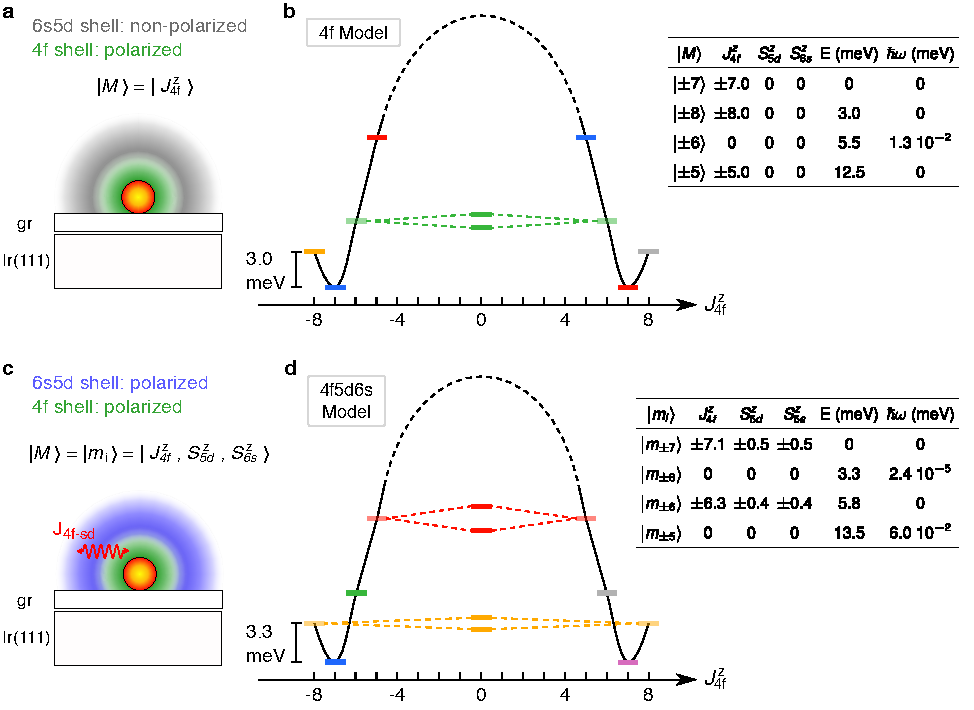
\includegraphics[width=0.98\textwidth]{Fig1_new.pdf}
\caption{Comparison of the polarized and non-polarized models. \textbf{a-c}. Choice of basis and resulting level scheme for energies $E<20$ meV for the non-polarized model. \textbf{d-f}. The same as \textbf{a-c} for the polarized model. 
\label{fig:intra} }
\end{figure*}

We now describe the mechanisms by which the magnetization is driven out of the ground states $\ket{M}=\ket{\pm7}$ and into the higher energy states, in which QTM can occur. The intrinsic lifetime of the Dy system is limited by substrate electron and phonon scattering (Fig.~\ref{fig:no_tip_tip_telegraph}a), while the measured lifetime is determined by additional electron scattering channels and any stray magnetic field due to the presence of the STM tip (Fig.~\ref{fig:no_tip_tip_telegraph}b).  We assume that the spins grafted on the graphene experience the effect of a two-dimensional phonon bath \cite{cervetti2016}. Phonons can be interpreted as a deformation of the substrate, perturbing the crystal field, and influencing only the external $4f$-shell, due to its non-vanishing orbital component (see supplemental for the Hamiltonian term). Phonons can induce transitions with $\Delta m = \pm 1$, and $\Delta m = \pm 2$ \citep{cervetti2016}, and they represent an efficient way for the de-excitation of the Dy adatom, from the excited states towards the ground states $\ket{m_{\pm 7}}$. From Refs.~\cite{politi_tunneling_1995, cervetti2016}, the transition rates between the states $\ket{M}$ and $\ket{M^{\prime}}$ write :

\begin{equation}
    \label{eq:phonon_rates}
    W_{MM^{\prime}}^{ph}=\dfrac{3 \nu_{ph}}{2\theta_{Dy}\rho_{gr}c_{gr}^4 \hbar^3} \mathcal{P} \left( E_{MM^{\prime}}, T \right) w^{ph}_{MM^{\prime}}
\end{equation}

in which $\nu_{ph}$ represents the phonon-spin coupling cross section, $c_{gr}$ is the speed of sound in graphene, $\rho_{gr}$ is the graphene density, $\theta_{Dy}$ is the Dy coverage referred to a graphene monolayer. $\mathcal{P}\left( E_{MM^{\prime}}, T \right)$ depends on the Bose-Einstein distribution at the sample temperature $T$ and on the energy difference $E_{MM^{\prime}}$ between the states $\ket{M}$ and $\ket{M^{\prime}}$. $w^{ph}_{MM^{\prime}}$ are the phonon matrix elements, calculated assuming that phonons act only on the external $4f$ shell (see Supplemental).
% \begin{align}
%     \label{eq:ph_abs}
%     W_{MM^{\prime}}^{ph} & =\dfrac{3 \nu_{ph}E_{MM^{\prime}}^2}{2\theta_{Dy}\rho_{gr}c_{gr}^4 \hbar^3}\dfrac{1}{e^{E_{MM^{\prime}}\beta}-1}w^{ph}_{MM^{\prime}}\\
%     W_{MM^{\prime}}^{ph} & =\dfrac{3 \nu_{ph} E_{MM^{\prime}}^2}{2\theta_{Dy}\rho_{gr}c_{gr}^4 \hbar^3}\left(\dfrac{e^{E_{MM^{\prime}}\beta}}{e^{E_{MM^{\prime}}\beta}-1}\right)w^{ph}_{MM^{\prime}}
%     \label{eq:ph_emis}
% \end{align}

%for the adsorption and emission of a phonon, respectively. In the equations, $\nu_{ph}$ is the only unknown parameter and it represents the phonon-spin coupling cross section, $c_{gr}$ is the speed of sound in graphene, $\rho_{gr}$ is the graphene density, $\theta_{Dy}$ is the Dy coverage referred to a graphene monolayer, $\beta=1/k_bT$ and $T$ is the sample temperature. $E_{MM^{\prime}}$ represents the energy difference between the states $\ket{M}$ and $\ket{M^{\prime}}$, and it is equal to the zero-field splitting $\omega$ when there is no external magnetic field. $w^{ph}_{MM^{\prime}}$ are the matrix elements, they are calculated assuming that phonons act only on the external $4f$ shell (see Supplemental).
The other contribution limiting the spin-lifetime of the Dy adatoms without the influence of the STM tip is the scattering with the substrate electrons, represented by $e^{-}_{SS}$ in Fig.\ref{fig:no_tip_tip_telegraph}a. The creation or annihilation of an electron hole pair in the substrate induces a spin transition ($\Delta m=\pm 1$) in the external \textit{6s-5d} shell \cite{}"loth paper about tunneling through ext shells". Consequently, the magnetic moment of the $4f$ shell flips, because the intra-atomic exchange interaction forces the magnetization alignment of the coupled internal and external shells \cite{pivetta2020}. We consider a non-polarized substrate, so that substrate electrons scattering bolsters an equal occupation of the doubly degenerate ground state.\newline
\indent We can introduce the terms coming from the STM tip to describe SP-STM experimental conditions.
%, as sketched in Fig.~\ref{fig:no_tip_tip_telegraph}b. 
In SP-STM experiments, we use an anti-ferromagnetic MnNi tip to measure the magnetization state of an isolated Dy adatom via magnetoresistive effect \cite{wiesendanger_ObservationVacuumTunneling_1990,Khajetoorians2013,paul_ControlMillisecondSpin_2017,Natterer2017,Natterer2018}. The fixed spin-polarization of the tip enables the measurement of the spin-lifetimes of the ground-states $\ket{m_{\pm7}}$, the spin-lifetimes of the excited states being too short to be detected within the bandwidth of available current-sensing electronics.


Fig.~\ref{fig:no_tip_tip_telegraph}c shows an example of telegraph-noise signal (TNS) traces at positive tip-sample voltage bias $V_b$ in which the tunneling current switches between a high-conductance (HC) and low-conductance (LC) state, corresponding to matching or opposite alignement between the spin-polarization of the tip and the magnetization of the adatom, respectively \cite{delgado2010,paul_ControlMillisecondSpin_2017}. 
From a TNS trace we extract two quantities: the occupancy, defined as the fraction of time that the magnetization adatom is in the high-conductance (HC) or low-conductance (LC) state, and the characteristic time $\tau ^*=(\tau_{HC}  \cdot \tau_{LC})/( \tau_{HC} + \tau_{LC})$, defined by the average HC and LC state lifetimes, $ \tau_{HC}$ and  $\tau_{LC}$, respectively \cite{Khajetoorians2013} (see supplemental). 


%brief description of the experiments
The mechanisms determining the spin-lifetimes of Dy adatoms in SP-STM measurements, \textit{i.e.} we account for the influence of the STM tip, are sketched in Fig.~\ref{fig:no_tip_tip_telegraph}b.
Firstly, magnetic tips in tunneling distances from an adatom generates a magnetic field which can span from the mT range to 10 T \cite{yang2019}. The exchange component can have a non-trivial dependence from the tip-adatom distance and can change due to atomic-scale modifications of the tip termination \cite{hauptmannQuantifyingExchangeForces2020,tao_SwitchingSingleSpin_2009,lazoFirstprinciplesStudyMagnetic2011,lazoRoleTipSize2008,wieserTheoreticalStudyDynamical2013}. The out-of-plane component of the tip field $B_{tip}$ used in the model is in the 100-900 mT range, depending on the tip-sample distance and it is chosen to give the best agreement between theory and experiments (see supplemental for further details).
\begin{figure*}[ht!]
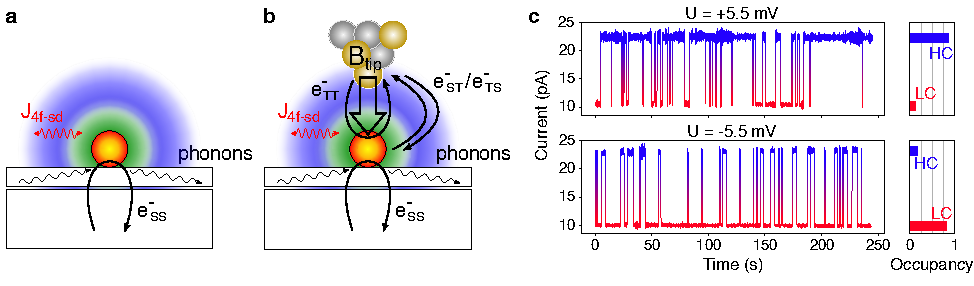
\includegraphics[width=0.98\textwidth]{Fig2_new.pdf}
\caption{Intra-atomic vs no intra-atomic
\label{fig:no_tip_tip_telegraph} }
\end{figure*}
%Firstly, the magnetic tip generates a magnetic field having a dipolar $B_{dip}$ and an exchange $B_{ex}$ contribution. The relative strength of the two components depends on the tip-adatom distance $d_{TS}$ \cite{willke}. 
% The tip field is defined by the dipolar $B^0_{dip}$ and exchange $B^0_{ex}$ component at a tip-sample distance of $d_{TS}=5$ \AA (see supplemental). The dipolar field scales with $1/d_{TS}^3$ and acts on all the polarized shell. For simplicity, we consider the exchange contribution to have a pure exponential dependence on tip-sample distance, $\propto e^{-d_{TS}/\lambda_{ex}}$, where $\lambda_{ex}$ is the exchange decay length \cite{}.
% As the exchange interaction is a function of the superposition between the tip and adatom electronic wavefunctions, we assume that the exchange tip field component acts only on the external \textit{6s-5d} shell.
%  which acts on the polarized shells proportionally to their magnetic moment and an effective g-factor (see Supplemental).
The tip field shifts the magnetic states via Zeeman effect lifting the degeneracy of the magnetic states sitting on the opposite side of the MAE barrier. This induces an energetically preferred ground-state, which can be related to the asymmetry in the occupation of $\ket{m_7}$ and $\ket{m_{-7}}$ states observed experimentally.
%The ground states $\ket{m_{\pm7}}$  are shifted apart in energy, lifting the degeneracy. 
In second place, we consider the scattering with tip electrons, indicated by $e^{-}_{TT}$ in Fig.~\ref{fig:no_tip_tip_telegraph}a. An electron originating in the tip can transfer its energy and momentum to an external Dy electron ($\Delta m=\pm 1$), eventually tunneling back to the tip. The magnetic tip used in SP-STM experiments can be characterized by a spin-up $\rho_{T\uparrow}$ and spin-down $\rho_{T\downarrow}$ populations at the Fermi level. The asymmetry in the population engenders a higher probability of spin-increasing ($\Delta m=+1$) or spin-decreasing ($\Delta m=-1$) transitions in the Dy adatom, respectively. Note that neither $e^{-}_{SS}$ nor $e^{-}_{TT}$ electrons contribute to the tunneling current, but they do affect the spin dynamics of the system. Finally, we consider the interaction with tunneling electrons, $e^{-}_{TS}$ and $e^{-}_{ST}$ in Fig.~\ref{fig:no_tip_tip_telegraph}b. A fraction of these electrons do not exchange their momentum with the Dy adatom, and they constitute the elastic contribution to the current. The electrons interacting with the atomic spin induce spin transitions and build up the inelastic contribution to the tunneling current. The tip spin-polarization reflects determines the proportion between spin-increasing and spin-decreasing transitions induced by the inelastic current. Formally, the coupling between adatom and electrodes, \textit{i.e.} the tip and the substrate, is modeled by a Kondo-type Hamiltonian \cite{delgado2010,delgadoSpinTransferTorqueSingle2010,fern2009} (see Supplemental). The transition rates associated with sample-to-sample ($e^{-}_{SS}$), tip-to-tip ($e^{-}_{TT}$), tip-to-sample ($e^{-}_{TS}$) and sample-to-tip ($e^{-}_{ST}$) can be compactly written as:
% \begin{equation}
%  \begin{split}
%     W_{MM^{\prime}}^{\eta}=\sum_{a=+,-,z} w_{MM^{\prime}}^a \dfrac{2\pi}{\hbar} \zeta^2 \left( &\varsigma_{\eta}\varsigma_{\eta^{\prime}} Q_{\eta \eta^{\prime}}^a \mathcal{F}_{\eta \eta^{\prime}}(E_{MM^{\prime}},U)\\
%      & +\varsigma_{\eta}^2  Q_{\eta \eta}^a  \mathcal{F}_{\eta \eta}(E_{MM^{\prime}}) \right)
%  \end{split}
% \end{equation}

\begin{equation}
    W_{MM^{\prime}}^{\eta}=\dfrac{2\pi}{\hbar} \zeta^2 \varsigma_{\eta} \left( K_{\eta \eta^{\prime}}+ K_{\eta \eta} \right)w_{MM^{\prime}}^{el}, \qquad \eta,\eta^{\prime}=T,S
    \label{eq:elec_rates}
\end{equation}

in which $w_{MM^{\prime}}^{el}$ are the matrix elements describing the interaction with the external $6s-5d$ electrons, $\varsigma_{\eta}$ is the coupling with the electrode $\eta$, $\zeta$ is the ratio between inelastic and elastic tunneling matrix elements, that we assume to be the same for tip and sample. $K_{\eta \eta^{\prime}}$ accounts for the scattering from the tunneling electrons ($e^{-}_{TS}$, $e^{-}_{ST}$) , while $K_{\eta \eta}$ is the analogous for the electrons originating and ending in the same electrode ($e^{-}_{SS}$, $e^{-}_{TT}$) and they are a function of $V_b$ and $T$ (see Supplemental).


% they are defined as:
% \begin{align}
%     &K_{\eta \eta^{\prime}}=\varsigma_{\eta^{\prime}} \rho_{\eta \eta^{\prime}}\mathcal{F}_{\eta \eta^{\prime}}(E_{MM^{\prime}},U,T) \\
%     &K_{\eta \eta}=\varsigma_{\eta} \rho_{\eta \eta}\mathcal{F}_{\eta \eta}(E_{MM^{\prime}},0,T) 
% \end{align}

% in which $\rho_{\eta \eta^{\prime}}$ and $\rho_{\eta \eta}$ are the convoluted spin-dependent populations, while $\mathcal{F}_{\eta \eta^{\prime}}(E_{MM^{\prime}},U,T)$ and $\mathcal{F}_{\eta \eta}(E_{MM^{\prime}},0,T)$ include the Fermi distribution of the electrons at temperature $T$, and they depend on the bias voltage between tip and sample $U$ (vanishing for $e^{-}_{SS}$ and $e^{-}_{TT}$ electrons) and on the energy separation $E_{MM^{\prime}}$ between the states involved in the transition.

%To determine the contributions of the previous mechanisms acting in the spin dynamics of Dy/Gr/Ir(111), we have determined spin-lifetimes and occupancy from telegraph-noise traces measured as a function of bias $U$, temperature $T$, and current $I_{set}$. 

The transition rates in Eqs.~\ref{eq:phonon_rates} and~\ref{eq:elec_rates} can be used to solve master equations \cite{delgado2010,Khajetoorians2013,loth2010,cervetti2016} and obtain the model values for$\tau^*$ and the occupancy for a certain set of bias voltage $V_{b}$, temperature $T$, and current $I_{set}$. 


% We employ the model just presented to reproduce the spin-lifetimes and the occupancy extrapolated from telegraph-noise traces, similar to those in Fig. \ref{fig:no_tip_tip_telegraph}c, that we measure as a function of bias $V_{b}$, temperature $T$, and current $I_{set}$. The calculated values are obtained by solving the following master equations, using the transition rates in Eqs.~\ref{eq:phonon_rates} and \ref{eq:elec_rates}:
% \begin{align}
% %\dfrac{dP_M}{dt}= & -P_M \sum_{M\neq M^{\prime}}\left[ \left(  W_{MM^{\prime}}^{\eta} \right) +P_{M^{\prime}}\left(  W_{M^{\prime}M}^{\eta} \right) \right] + Q_M^{QTM} \left(P_{-M}- P_{M} \right)
% \begin{split}
% \dfrac{dP_M}{dt}=&-P_M \sum_{M\neq M^{\prime}}\left(   W_{MM^{\prime}}^{tot}  +P_{M^{\prime}}  W_{M^{\prime}M}^{tot}  \right) \\
% %&+ Q_M \left(P_{-M}- P_{M} \right)
% \end{split}
% \end{align}

% in which $P_M$ is the population of the state $M=\ket{m_i}$ $W_{MM^{\prime}}^{tot}=W_{MM^{\prime}}^{ph}+W_{MM^{\prime}}^{T}+W_{MM^{\prime}}^{S}$ is the sum of the phonon and electron transition rates. The inclusion of quantum tunneling rates as in Refs. [] do not affect the spin-dynamics of the system in the present case (see supplemental).
%, and $Q_M$ are transition rates associated to quantum tunneling of magnetization between states $M=\ket{m_i}$ and $-M=\ket{m_{-i}}$ \cite{} (see supplemental).
We optimize the value of the free parameters describing the tip field $B_{tip}$, the spin-phonon coupling ($\nu_{ph}$) and the interaction with electrons ($\zeta$, $\varsigma_{\eta}$) to get the best agreement with experimental data.

%Fig.~\ref{fig:bias}a shows the occupancy and spin-lifetimes for the bias dependent measurements. At high energy ($\pm$8 mV), we observe a clear spin-torque effect, in which tip polarization forces the adatom in the HC and LC state, at positive and negative bias, respectively. This effect is also clearly visible in the two telegraph-noise signal traces shown in Fig.~\ref{fig:no_tip_tip_telegraph}c. At lower positive bias, the asymmetry shrinks, while at negative bias there is a crossing in the occupancy at $\sim$ -5 mV. The strong spin-pumping effect observed at $U>4$ mV and $U<-4$ mV comes with a rapid decrease of the spin lifetimes, as observed in Fig.~\ref{fig:bias}b. According to our model, the intra-atomic exchange strongly mixes the $\ket{m_{\pm 5}}$ states at 3.3 meV, and the $\ket{m_{\pm 8}}$ states at 13.5 meV, opening two QTM channels for magnetization reversal. Thus, the spin dynamics of the Dy adatoms in the 0-10 mV range is determined by the activation of the $\ket{m_{\pm 7}} \rightarrow \ket{m_{\pm 8}}$  and $\ket{m_{\pm 7}} \rightarrow \ket{m_{\pm 6}} \rightarrow \ket{m_{\pm 5}} $ excitation pathways, see Fig.~\ref{fig:bias}d. These processes superimpose in Fig.~\ref{fig:bias}a, because of the temperature ($T=6.5$ K) which smears out the transitions. To better understand the effects of the temperature and polarization in our model, we show in Fig.~\ref{fig:bias}c the comparison of the occupancy as a function of bias at two temperatures and two values of the tip polarization. In the case of $T=1$ K and 100\% tip polarization, we observe that at low positive bias ($U<1$ mV), the HC state is preferred. At these energies, the spin lifetimes are determined by thermal-asssisted excitations from the ground-states $\ket{m_{\pm 7}}$ towards the first excited states, \textit{i.e.} $\ket{m_{\pm 8}}$. During these processes the external electrons of the Dy adatom exchange momentum with the substrate electrons ($e^{-}_{SS}$) and phonons. The asymmetry, on the other hand, is determined by the tip field which acts via Zeeman effects, favoring the occupation of the $\ket{m_{+7}}$ ground-state. Starting at 2 mV, the pumping due to tunneling electrons ($e^{-}_{TS}$) becomes stronger, as we approach the energy value of the first transition, \textit{i.e.} $E_{\ket{m_{\pm 7}}\ket{m_{\pm 8}}}$=3.3 meV. The polarization of the tip ($\rho_{T\uparrow}$=0.7) promotes spin in

Fig.~\ref{fig:bias}a and b show the occupancy and spin-lifetimes measured as a function of bias and the corresponding polarized model prediction at $T=6.5$ K. The processes that determine the trends in occupancy can be characterised into three regimes. To better elucidate these regimes, Fig.~\ref{fig:bias}c displays the polarized model prediction at $T=1$ K. For biases between $\pm 2$ meV (white in Fig.~\ref{fig:bias}c), the majority occupation is limited to the ground states, and occupancy is primarily determined by the tip field $B_{tip}$ through Zeeman splitting. The tip field produces an asymmetric occupation in competition with the substrate electrons ($e^{-}_{SS}$) and phonons that yield symmetric occupation due to their non-polarized nature. At biases between $+2$  and $+6$ meV (yellow in Fig.~\ref{fig:bias}c-d), transitions between the ground state $\ket{m_{+7}}$ and first excited state $\ket{m_{+8}}$ occur, allowing for magnetisation reversal through QTM via $\ket{m_{\pm 8}}$. For $\rho_{T \uparrow} > 0.5 $, the high-conductance state corresponds to positive $\ket{m_{+i}}$ states, and tip-to-substrate tunnelling is dominated by spin-increasing transitions. Fig.~\ref{fig:bias}d illustrates the transition pathway allowed at these energies, resulting in a low-conductance preferred state corresponding to the negative $\ket{m_{-i}}$ states. The situation is reversed at biases between $-2$  and $-6$ meV. Substrate-to-tip tunnelling is dominated by spin-decreasing transitions, thus a high-conductance state corresponding to the positive $\ket{m_{+i}}$ states is preferred. 
Note that if the spin polarization of the tip is reversed, this situation remains the same. For example, if $\rho_{T \uparrow} < 0.5 $, the high-conductance state now corresponds to negative $\ket{m_{-i}}$ states, tip-to-substrate tunnelling is dominated by spin-decreasing transitions, and a low-conductance state corresponding to the positive $\ket{m_{+i}}$ states is preferred. At biases above $+6$ meV (red in Fig.~\ref{fig:bias}c-d), transitions between the ground states $\ket{m_{\pm7}}$ and higher excited states $\ket{m_{\pm 6, \pm 5}}$ occur, allowing for magnetisation reversal through QTM via $\ket{m_{\pm 5}}$. For $\rho_{T \uparrow} > 0.5 $, tip-to-substrate tunnelling is still dominated by spin-increasing transitions. The resulting transition pathway is pictured in Fig.~\ref{fig:bias}d. This results in a preferred high-conductance state corresponding to the positive $\ket{m_{+i}}$ states. The degree of tip polarization determines how dominant the spin-increasing or spin-decreasing processes are within a given bias range. For $\rho_{T \uparrow} = 1$, only one process is possible, and the occupancy saturates to either 0 or 1 depending on the transition pathway and tunnelling direction. For $\rho_{T \uparrow} < 1$, the spin-increasing and spin-decreasing processes compete. In the regime above $\pm 6$ meV, the tip polarization determines the saturation occupancy. At higher temperatures, the delineation between the regimes is smear, resulting on the trend observed in Fig.~\ref{fig:bias}c. 

\begin{figure*}[ht!]
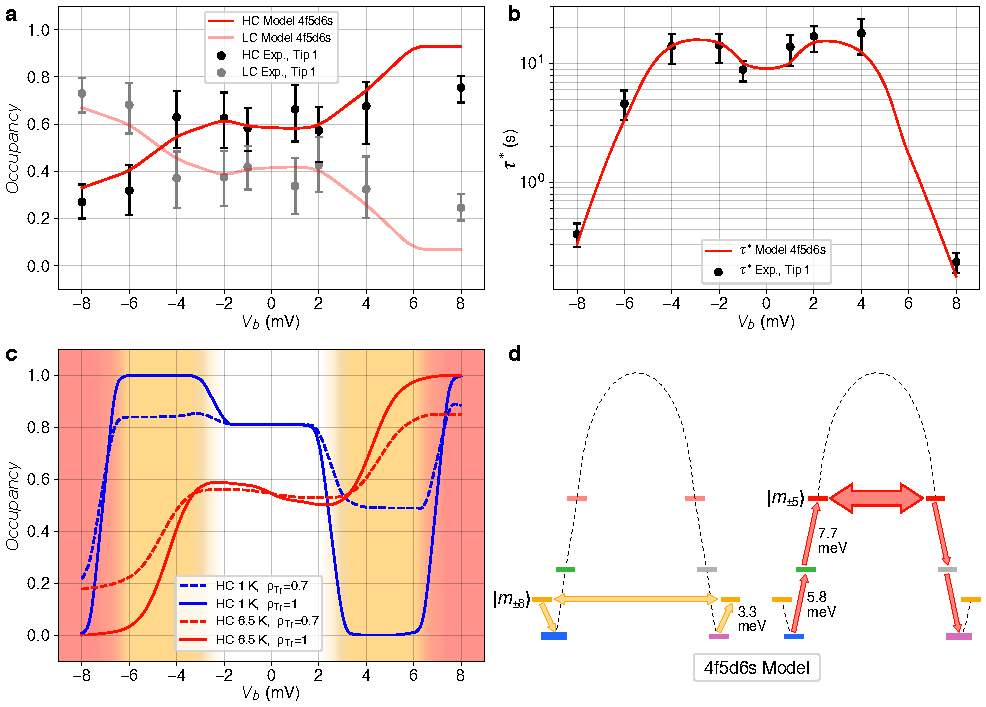
\includegraphics[width=0.99\textwidth]{Fig4_new.pdf}
\caption{Variable Bias Measurements
\label{fig:bias} }
\end{figure*}

% The ratio $\zeta$ and the coupling to the electrodes $\varsigma_T$, $\varsigma_S$ are treated as free-parameters. We assume that the coupling to the surface $\varsigma_S$ is constant and that it does not depend on the position in the Moiré pattern the adatom is sitting. The coupling to the tip $\eta_T$ scales with the set tunneling current. We define $I_0$ as the average between the high-conductance (HC) and low-conductance (LC) current, see Fig.~\ref{fig:no_tip_tip_telegraph}c. By neglecting the inelastic contribution to this current, which is orders of magnitudes lower than the elastic one, we can relate $\eta_T$ to $\eta_S$ using the experimental value of $I_0$:

% \begin{equation}
%   \varsigma_T= \dfrac{4 \hbar I_0}{2\pi e [f(U,T)-f(-U,T)]\varsigma_S (\rho_{S\uparrow} \rho_{T\uparrow} + \rho_{S\downarrow} \rho_{T\downarrow})}
% \end{equation}

% where $e$ is the electron charge and $f$ is the Fermi-Dirac distribution.

\begin{figure*}[h!]
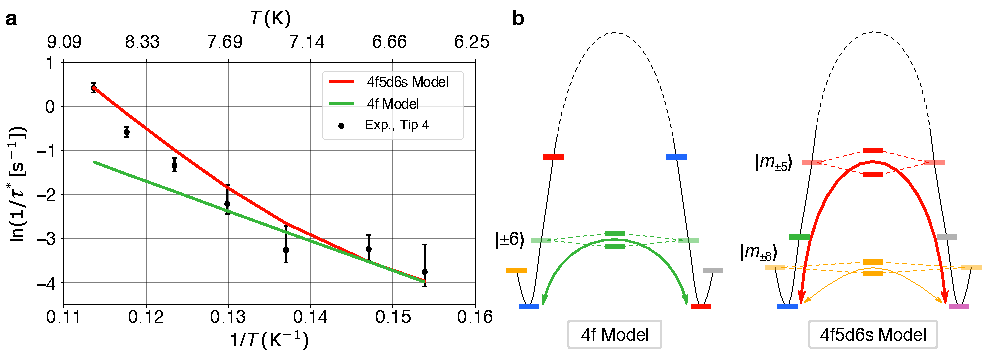
\includegraphics[width=0.99\textwidth]{Fig3_new.pdf}
\caption{Variable Temperature Measurements. \textbf{a}. Arrhenius plot comparing the polarized (red) and non-polarized (green) models with the experimental observations (black). \textbf{b}. Level scheme of the two models. The slope of the Arrhenius is determined by the height of the anisotropy barrier, and therefore manifest the differences in the reversal pathways between each model. 
\label{fig:temp} }
\end{figure*}
Fig.~\ref{fig:current} shows the spin-lifetimes for the temperature dependent measurements, taken at $V_{b} = +1$ mV.


\begin{figure*}[h!]
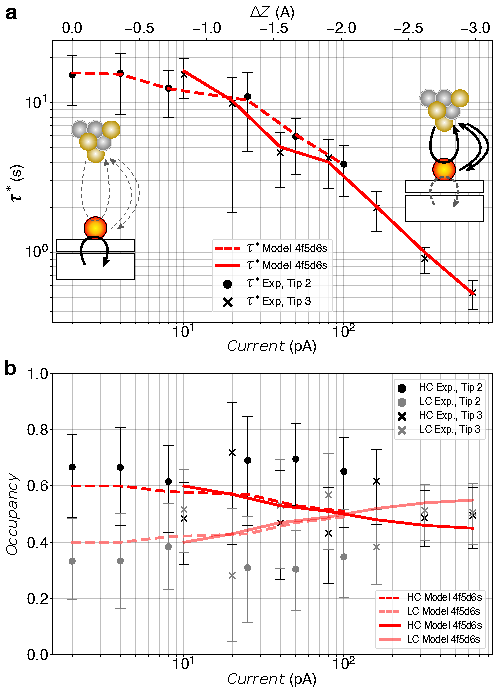
\includegraphics[width=0.5\textwidth]{Fig5_new.pdf}
\caption{Variable Current Measurements. \textbf{a}. Lifetime measurements as a function of set-point current and corresponding $\Delta Z$ ($\AA$) distance ($V_{b} = +1$ mV, $T = 6.5$ K). $\Delta Z = 0$ is fixed by the lowest current point. \textbf{b}. Occupancy measurements for each point in \textbf{a}.
\label{fig:current} }
\end{figure*}

Fig.~\ref{fig:current} shows the occupancy and spin-lifetimes for the current dependent measurements, taken at $V_{b} = +1$ mV. A decreasing $B_{tip}$ is needed to reproduce the experimental data (see Supplementary). In the low current regime, substrate-substrate electron scattering $e^{-}_{SS}$, phonon scattering, and the tip field $B_{tip}$ are the dominant mechanisms that determine state occupancy and lifetime. The tip field is aligned with the majority spin state at the Fermi level, evidenced by the preferred high-conductance state (Fig.~\ref{fig:current}b). As the current is increased, and the tip is moved closer to the Dy adatom, tip-substrate $e^{-}_{TS}$ and tip-tip electron scattering $e^{-}_{TT}$ play a larger role and compete with the aforementioned mechanisms. As described in the variable bias measurements, the spin increasing processes that dominate tip-substrate scattering at low positive biases result in a preferred low-conductance state via the transition pathway between the $\ket{m_{8}}$ and $\ket{m_{-8}}$ states. Due to the increasing amount of tip-substrate scattering events, this process begins to dominate the tip field at currents greater than $100$ pA, resulting in a preferred low-conductance state in the high current regime. 


\bibliographystyle{unsrt}
\bibliography{bib.bib}

\end{document}

